\documentclass{beamer}
\beamertemplatenavigationsymbolsempty
\usecolortheme{beaver}
\setbeamertemplate{blocks}[rounded=true, shadow=true]
\setbeamertemplate{footline}[page number]
%
\usepackage[utf8]{inputenc}
\usepackage[english, russian]{babel}
\usepackage{amssymb,amsfonts,amsmath,mathtext}
\usepackage{subfig}
\usepackage[all]{xy} % xy package for diagrams
\usepackage{array}
\usepackage{multicol}% many columns in slide
\usepackage{hyperref}% urls
\usepackage{hhline}%tables
\usepackage{algorithm}
\usepackage{algpseudocode}
\usepackage{dashbox}
\usepackage[most]{tcolorbox}


\setlength{\columnsep}{1cm}

\usepackage{setspace}

\newcommand{\advisor}[1]{\gdef\@advisor{#1}}
\newcommand{\printadvisor}{\@ifundefined{@advisor}{}{\textbf{Advisor:} \@advisor}}

\newcommand{\supervisor}{\small Научный руководитель: Бахтеев Олег (кандидат ф-м наук)}


% Your figures are here:
\graphicspath{{./figures}}

%----------------------------------------------------------------------------------------------------------
\title[\hbox to 56mm{Feature generation}]{Поиск архитектуры смеси экспертов с помощью суррогатной модели}
\author[~Babkin]{Бабкин Пётр}
\institute{}
\date{}

%----------------------------------------------------------------------------------------------------------
\begin{document}
%----------------------------------------------------------------------------------------------------------
\begin{frame}
    \thispagestyle{empty}
    \maketitle
    \vspace{-2.3cm}
    \centering
    %\small Научный руководитель: к.ф.-м.н. Бахтеев Олег

    \vspace{0.6cm}

Кафедра интеллектуальных систем ФПМИ МФТИ

Специализация: Интеллектуальный анализ данных

Направление: 03.04.01 Прикладные математика и физика

\bigskip

2026

\end{frame}
%-----------------------------------------------------------------------------------------------------
\begin{frame}{План работы}
    \begin{block}{Цель исследования:}
        Предложить метод поиска архитектуры для смеси экспертов.
    \end{block}
    \begin{block}{Проблема:}
        Адаптация методов поиска архитектуры нейронной сети для задачи поиска архитектуры смеси экспертов неэффективна: сложность поиска растет линейно с числом экспертов.
    \end{block}
    \begin{block}{Предлагаемый метод:}
        Предлагается оценивать качество архитектур каждого из экспертов с помощью суррогатной функции.
        Суррогатная функция обучается одновременно с оптимизацией назначений экспертов и поиска архитектур.
    \end{block}
\end{frame}
%----------------------------------------------------------------------------------------------------------
\begin{frame}{Постановка задачи}
    \begin{block}{Максимизация правдоподобия смеси экспертов}
        \vspace{-8mm}
        \begin{gather*}
            \prod_{n=1}^{N} \sum_{k=1}^{K} p(y_n, n \in C_k \mid x_n, \alpha_k, \theta_k) \to \max_{\alpha_1, \dots, \alpha_K, \theta_1, \dots, \theta_K},
        \end{gather*}
        где $K$ -- кол-во экспертов, $N$ -- кол-во элементов данных. Для $k$-ого эксперта $C_k$ -- его индексы данных, $\theta_k$ -- параметры, $\alpha_k$ -- архитектура.
    \end{block}

    \begin{block}{Задача поиска архитектуры смеси из $K$ экспертов}
    \vspace{-5mm}
    \begin{gather*}
        \prod_{n=1}^{N}\sum_{k=1}^{K} r_{nk}\, u(\alpha_k, R_k) \to \max_{\alpha_1,\ldots,\alpha_K,\, R_1,\ldots,R_K},
    \end{gather*}
    где $r_{nk}$ --- вероятность назначения элемента $n$ эксперту $k$, $R_k = \{r_{nk}\}_{n=1}^{N}$, $u(\alpha_k, R_k)$ --- суррогатная функция, оценивающая качество архитектуры $\alpha_k$ на данных $R_k$.
    \end{block}

\end{frame}
%----------------------------------------------------------------------------------------------------------
\begin{frame}{Схема работы}
    Архитектуры экспертов и кластеры данных подбираются для каждого кластера с помощью суррогатной модели $u$.
    \begin{figure}
        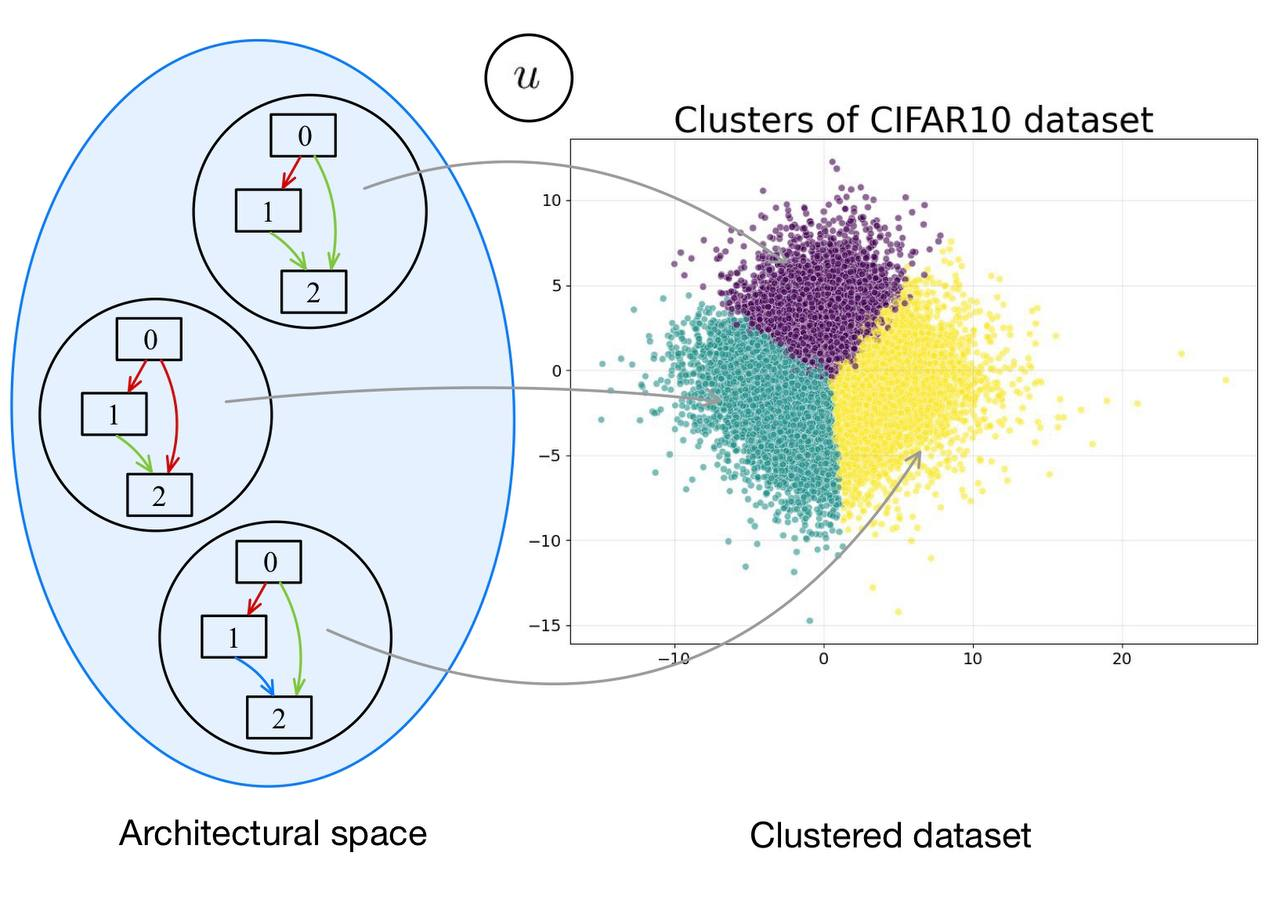
\includegraphics[scale=0.22]
        {method}

    \end{figure}

\end{frame}
%----------------------------------------------------------------------------------------------------------
\begin{frame}{Суррогатная модель для оценки качества экспертов}

    Суррогатная функция $u(\alpha, R)$ предсказывает валидационную точность архитектуры $\alpha$ на данных, определяемых вектором $R$:
    $$u: \mathcal{A} \times \{0,1\}^N \to \mathbb{R},$$
    где $\mathcal{A}$ -- пространство архитектур.

    \bigskip

    Суррогат представляет собой нейронную сеть или Гауссовский процесс, который обучается на триплетах $(\alpha, b, a)$, где $b \in \{0,1\}^N$, $a$ -- точность архитектуры, обученной на данных, соответствующих $b$.

\end{frame}
%----------------------------------------------------------------------------------------------------------
\begin{frame}{Предлагаемый метод}

 Обобщенный EM-алгоритм с использованием суррогатной функции.

\begin{figure}[h]
  \begin{minipage}{1.\linewidth}
    \begin{algorithm}[H]
    \caption{SGEM}\label{alg:em}
        \begin{algorithmic}[1]
            \State \textbf{Вход:} $K$, данные, кластеризация, $u^{(0)}$ --- начальный суррогат
            \For{$t = 0, 1, 2, \ldots$}
                \State \textbf{E-шаг:} $q_{mk}^{(t)} \sim r_{mk}^{(t)}\, u^{(t)}(\alpha_k^{(t)}, R_k^{(t)})$
                \State \textbf{M-шаг:} $\sum_m \sum_k q^{(t)}_{mk} \log\left(r_{mk} u^{(t)}(\alpha_k, R_k)\right) \to \max_{\overline{\alpha}, \overline{R}}$
                \State \textbf{S-шаг:} добавить актуальные данные, переобучить $u$
            \EndFor
        \end{algorithmic}
    \end{algorithm}
  \end{minipage}
\end{figure}

\bigskip

\textbf{Градиентный метод}: вместо E/M-шагов --- прямая градиентная оптимизация $r$ и $\alpha$.

\end{frame}
%----------------------------------------------------------------------------------------------------------
\begin{frame}{Сходимость GEM с адаптивным суррогатом}
    \begin{tcolorbox}[
    colback=gray!10, colframe=gray!50, arc=5mm,
    boxsep=0.5mm, left=3mm, right=3mm, top=2mm, bottom=2mm
    ]
    \textbf{Теорема.} Пусть $\{\theta^{(t)} = (\alpha^{(t)}, r^{(t)})\}_{t=1}^\infty$ --- последовательность GEM-алгоритма с суррогатом $u^{(t)}$, и выполнены условия: (1)~равномерная ограниченность $u_{\mathrm{true}}$ и $\{u^{(t)}\}_{t=1}^\infty$, (2)~$\sum_{t=1}^\infty \varepsilon_t < \infty$ где $\varepsilon_t = \sup |\log u^{(t)} - \log u_{\mathrm{true}}|$, (3)~на $M$-шаге $\mathcal{F}$-функция не убывает, (4)~$u(\alpha, r)$ непрерывно по второму аргументу $\forall \alpha \in \mathcal{A}$. Тогда:

    \medskip
    \textbf{(a)} $\{L_{\mathrm{true}}(\theta^{(t)})\}$ сходится.

    \textbf{(b)} Любая предельная точка $\theta^{\star}$ является стационарной:
    $Q_{\mathrm{true}}(\theta;\, \theta^{\star}) \leq Q_{\mathrm{true}}(\theta^{\star};\, \theta^{\star})$ для всех $\theta \in \Theta$, где $Q_{\mathrm{true}}(\theta;\, \theta') = \sum_m \sum_k w_{mk}(\theta')\, \log\!\bigl(r_{mk}\, u_{\mathrm{true}}(\alpha_k, R_k)\bigr)$ и $w_{mk}(\theta') = q_{mk}^{\star}(\theta')$.
    \end{tcolorbox}

    \medskip

\textbf{Замечание:} если $\varepsilon_t$ убывает экспоненциально с показателем $p > 1$, то $L_{\mathrm{true}}(\theta^{(T)}) \to L_{\mathrm{true}}(\theta^{\star})$ со скоростью $O(T^{1-p})$.    

\end{frame}
%----------------------------------------------------------------------------------------------------------
\begin{frame}{Цели вычислительного эксперимента}

    \begin{block}{Показать применимость метода}
        \begin{itemize}
            \item Проверить семантическую кластеризуемость реальных датасетов.
            \item Показать, что существует разброс точностей архитектур на разных кластерах данных.
        \end{itemize}
    \end{block}

    \bigskip

    \begin{block}{Проверить эффективность работы метода}
        \begin{itemize}
            \item Проверить эффективность методов для нахождения разбиения и архитектур на синтетических данных.
        \end{itemize}
    \end{block}

\end{frame}
%----------------------------------------------------------------------------------------------------------
\begin{frame}{Применимость метода}

    Существует разброс точности архитектуры по кластерам.

    \begin{columns}[c]
    \column{0.4\textwidth}
        \begin{figure}
            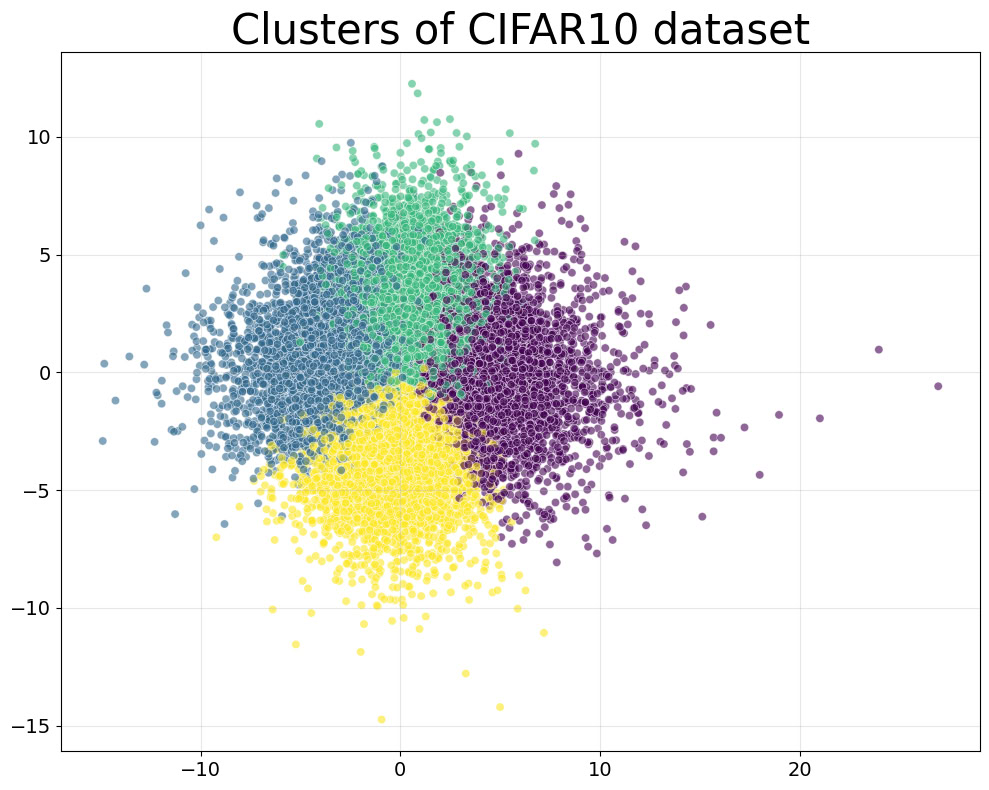
\includegraphics[scale=0.14]
            {clusters}
        \end{figure}

    \column{0.6\textwidth}
        \begin{figure}
            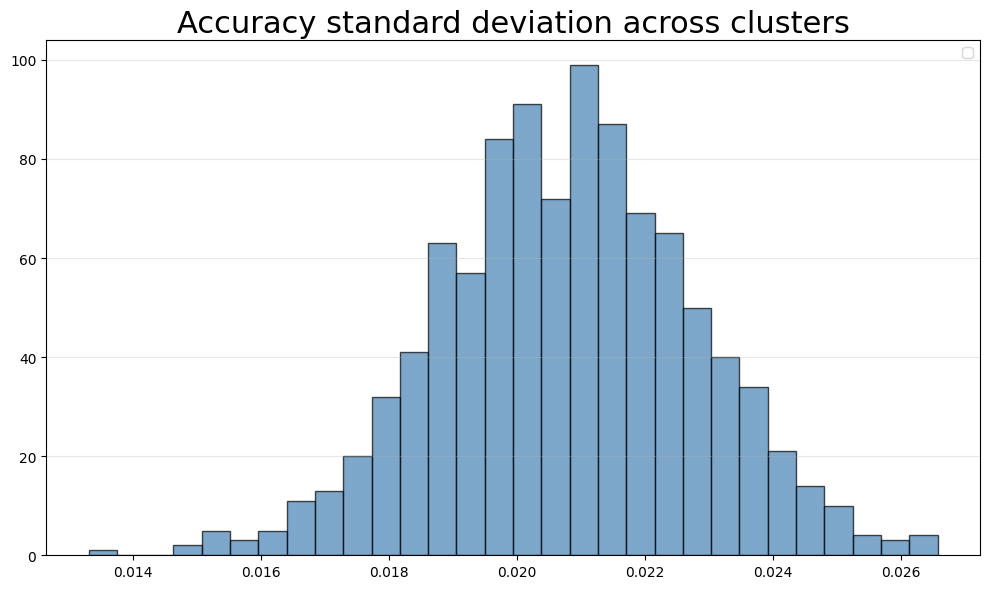
\includegraphics[scale=0.19]
            {acc_std}
        \end{figure}
    \end{columns}

    \bigskip

    Разброс в среднем составляет 2\%. Минимум он составляет 1,2\%.

\end{frame}
%----------------------------------------------------------------------------------------------------------
\begin{frame}{Эффективность работы}

    \begin{columns}[c]
    \column{0.5\textwidth}
        \begin{figure}
            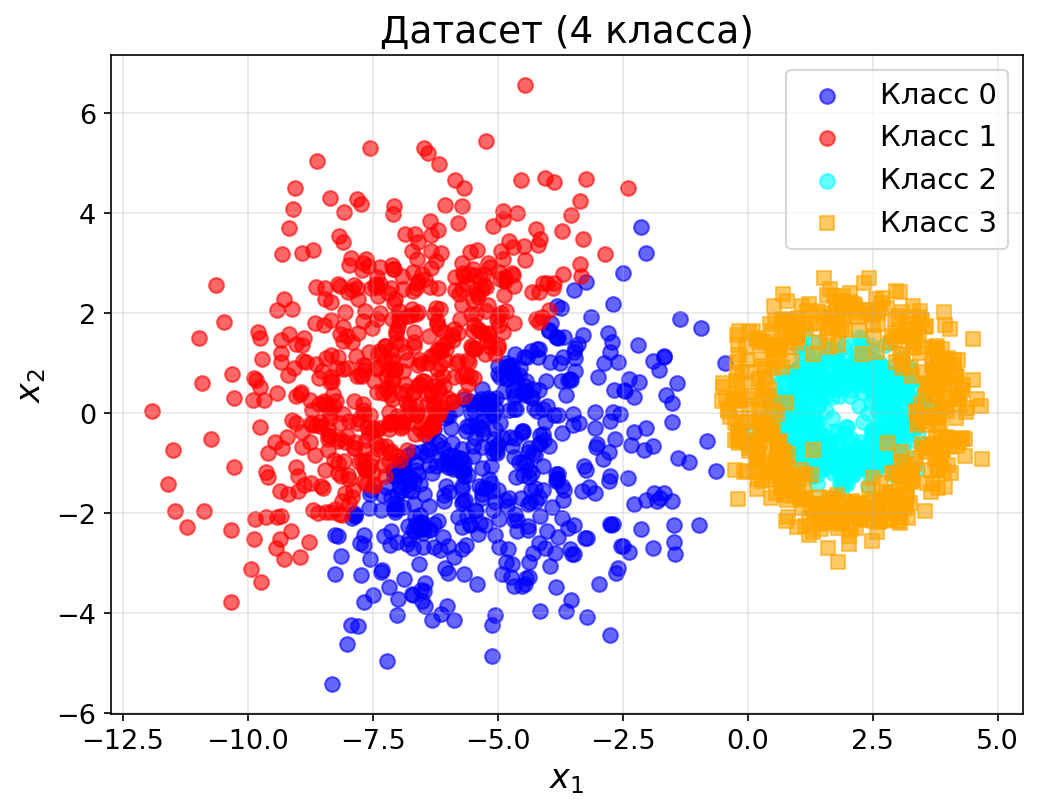
\includegraphics[width=\textwidth]{dataset}
        \end{figure}
    \column{0.5\textwidth}
        \begin{figure}
            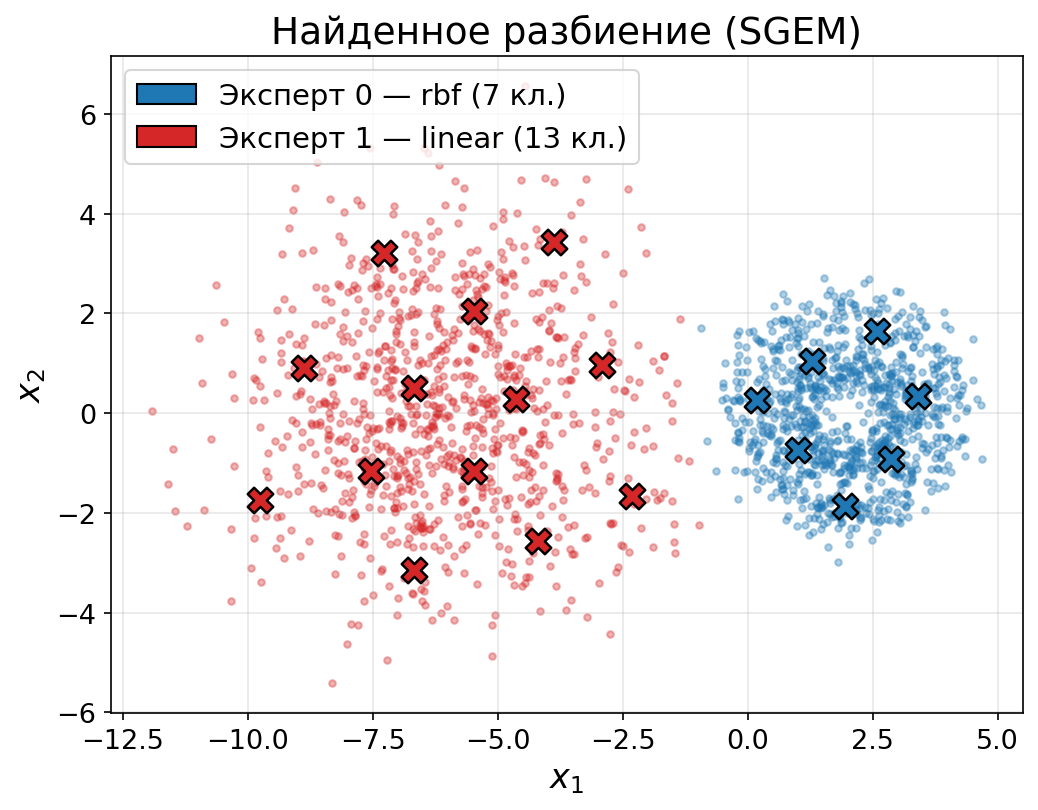
\includegraphics[width=\textwidth]{found_split}
        \end{figure}
    \end{columns}

    \vspace{-1mm}

    \begin{table}[h!]
    \centering
    \small
        \begin{tabular}{ |l|c|c|c| }
        \hline
        \textbf{Метод} & \textbf{Split} & \textbf{Совпадение} & \textbf{MoE acc} \\
        \hline
         SGEM & [7, 13] & \textbf{20/20} & \textbf{95.6\%}$^*$ \\
        \hline
         Единая архитектура & --- & --- & $\sim$75\% \\
        \hline
        \end{tabular}
    \end{table}

    \vspace{-2mm}
    \footnotesize $^*$С референсными архитектурами (linear + RBF) на найденном split.

\end{frame}
%----------------------------------------------------------------------------------------------------------
\begin{frame}{Заключение}
    \begin{block}{Достигнутые результаты:}
        \begin{itemize}
            \item Предложена постановка задачи для нахождения архитектуры смеси экспертов с помощью суррогатной функции
            \item Предложен метод SGEM для решения поставленной задачи
            \item Доказана теорема о сходимости GEM-алгоритма с адаптивным суррогатом
            \item В экспериментах алгоритм показал свою эффективность
        \end{itemize}
    \end{block}

    \begin{block}{Дальнейшая работа}
        \begin{itemize}
            \item Провести эксперименты на реальных датасетах (CIFAR, ImageNet)
            \item Сравнить с конкурирующими методами (AutoMoE, DSR)
            \item Исследовать масштабируемость метода на большое число экспертов
        \end{itemize}
    \end{block}
\end{frame}
%----------------------------------------------------------------------------------------------------------
\begin{frame}{Литература}
    \begin{itemize}
        \setlength\itemsep{0.7em}
        \small
        \item Chen Z. et al. Towards understanding mixture of experts in deep learning // arXiv:2208.02813, 2022.
        \item Jiang L. et al. AutoMoE: Heterogeneous mixture-of-experts with adaptive computation // ACL 2023.
        \item Piwko J. et al. Divide, specialize, and route: a new approach to efficient ensemble learning // arXiv:2506.20814, 2025.
        \item Dempster A.P. et al. Maximum likelihood from incomplete data via the EM algorithm // JRSS-B, 1977.
        \item Wu C.F.J. On the convergence properties of the EM algorithm // Annals of Statistics, 1983.
    \end{itemize}
\end{frame}
%----------------------------------------------------------------------------------------------------------
\end{document}
